% =====================================================================
%  Relativistic modification of Chapter XII, §111–112
%  Capillary instability of relativistic jets
% =====================================================================
%
%  Classical reference: Chandrasekhar, Ch. XII §111–112, eqs. (139)–(214)
%  Relativistic framework: SR perfect fluid + BDNK first-order causal dissipation
%  + relativistic resistive MHD for §112
%  Agent: 54
% =====================================================================

\section{Capillary instability of a relativistic liquid jet}
\label{sec:rel-111}

In the classical theory (\S\ref{sec:111}), the capillary instability of
a liquid jet of radius $R$ held together by surface tension $T$ was
analysed by Plateau and Rayleigh.  The key result is that
axisymmetric (varicose) perturbations with wavelength exceeding
the circumference $2\pi R$ are unstable, while all non-axisymmetric
modes are stable.  In this section we generalise the analysis to a
\emph{relativistic} jet in which the fluid satisfies the equations of
special-relativistic hydrodynamics.

The motivating physical context is provided by astrophysical jets
(active galactic nuclei, gamma-ray bursts, microquasars) where bulk
Lorentz factors $\Lf \gg 1$ are commonplace.  Even when the jet is
considered in its rest frame, relativistic corrections to the
equation of state and to the inertia enter whenever the internal
energy density $\varepsilon$ is not negligible compared to the rest-mass
energy density $\rho c^{2}$.

\subsection{Relativistic surface energy density}
\label{sec:rel-111-surface}

In the Newtonian treatment the surface tension $T$ (energy per unit
area) is a Galilean invariant.  In special relativity the surface
layer is described by a \emph{surface energy--momentum tensor}
\begin{equation}
\label{eq:rel-111-surface-emt}
S^{\mu\nu} = \sigma_{\mathrm{s}}\,
  \bigl(g^{\mu\nu} + n^{\mu}n^{\nu}\bigr)\Big|_{\Sigma},
\end{equation}
where $\sigma_{\mathrm{s}}$ is the \emph{relativistic surface energy
density} (rest-frame energy per unit proper area), $n^{\mu}$ is the
unit outward normal to the world-tube $\Sigma$ of the jet boundary,
and the tensor in parentheses projects onto the 2+1 dimensional
world-sheet.  In the rest frame of the surface element,
$\sigma_{\mathrm{s}}$ reduces to the classical surface tension $T$,
so
\begin{equation}
\label{eq:rel-111-sigma-rest}
\sigma_{\mathrm{s}} = T.
\end{equation}
For an observer boosted along the jet axis with Lorentz factor
$\Lf$, the surface energy density transforms as the $(0,0)$
component of $S^{\mu\nu}$, but the \emph{eigenvalue} $T$ is a
Lorentz scalar.  All stability calculations below are performed in
the jet rest frame, so $\sigma_{\mathrm{s}} = T$ throughout.

The Israel junction condition across the surface $\Sigma$ is
\begin{equation}
\label{eq:rel-111-junction}
\bigl[T^{\mu\nu}\bigr]\,n_{\nu}
  = -\nabla_{\alpha}\,S^{\mu\alpha},
\end{equation}
where $[\cdot]$ denotes the jump across $\Sigma$.  For a static
cylindrical equilibrium of radius $R$, the only non-trivial
component gives the relativistic Young--Laplace equation
\begin{equation}
\label{eq:rel-111-young-laplace}
p_{0} = \frac{T}{R},
\end{equation}
in exact agreement with the classical expression~\eqref{eq:12-140}.

\begin{relcorrection}
\textbf{Newtonian limit.}
The surface energy--momentum tensor~\eqref{eq:rel-111-surface-emt}
reduces to a simple surface tension when all velocities are
non-relativistic and the surface kinetic energy is negligible.
The junction condition~\eqref{eq:rel-111-junction} then reproduces
equation~X\,(24) of the classical text.
\end{relcorrection}

\subsection{Rayleigh--Plateau instability in special relativity}
\label{sec:rel-111-RP}

We consider a cylindrical jet of radius $R$ in its rest frame, with
equilibrium state characterised by uniform energy density
$\varepsilon_{0}$ (including rest-mass energy $\rho c^{2}$ and
internal energy), pressure $p_{0} = T/R$, and vanishing 3-velocity.
The relativistic enthalpy density is
\begin{equation}
\label{eq:rel-111-enthalpy}
\enthalpy \;=\; \frac{\varepsilon_{0}+p_{0}}{c^{2}}.
\end{equation}

Small perturbations about this state satisfy the linearised
relativistic Euler equations.  For an irrotational perturbation in
the jet rest frame, one introduces a velocity potential $\Phi$
through $\delta u^{i} = \partial^{i}\Phi$, and the linearised
continuity and momentum equations yield the relativistic wave equation
\begin{equation}
\label{eq:rel-111-wave}
\frac{1}{\cs^{2}}\,\frac{\partial^{2}\Phi}{\partial t^{2}}
  = \nabla^{2}\Phi,
\end{equation}
where the relativistic sound speed is
\begin{equation}
\label{eq:rel-111-cs}
\cs^{2} = \left(\frac{\partial p}{\partial\varepsilon}\right)_{\!s}
  \leq c^{2}.
\end{equation}
The inequality is the \emph{causality bound}: the sound speed must
not exceed the speed of light.

We seek normal-mode solutions of the form
\begin{equation}
\label{eq:rel-111-normalmode}
\Phi = \hat{\Phi}(\varpi)\,
  e^{i(kz + m\varphi) + \sigma t},
\end{equation}
where $(\varpi,\varphi,z)$ are cylindrical coordinates.
Substitution into~\eqref{eq:rel-111-wave} gives
\begin{equation}
\label{eq:rel-111-bessel}
\frac{d^{2}\hat{\Phi}}{d\varpi^{2}}
  + \frac{1}{\varpi}\frac{d\hat{\Phi}}{d\varpi}
  - \left(k^{2} + \frac{\sigma^{2}}{\cs^{2}}
    + \frac{m^{2}}{\varpi^{2}}\right)\hat{\Phi} = 0.
\end{equation}
Define the \emph{relativistically modified radial wave number}
\begin{equation}
\label{eq:rel-111-kperp}
\kappa^{2} = k^{2} + \frac{\sigma^{2}}{\cs^{2}}.
\end{equation}
In the Newtonian (incompressible) limit
$\cs \to \infty$, we have $\kappa \to k$ and recover the classical
modified Bessel equation.  The solution regular at $\varpi = 0$ is
\begin{equation}
\label{eq:rel-111-Phi-sol}
\hat{\Phi}(\varpi) = C\,I_{m}(\kappa\varpi),
\end{equation}
so the pressure perturbation inside the jet is
\begin{equation}
\label{eq:rel-111-deltap}
\frac{\delta p}{\enthalpy c^{2}} =
  -\sigma\,\hat{\Phi} = -C\sigma\,I_{m}(\kappa\varpi)\,
  e^{i(kz+m\varphi)+\sigma t}.
\end{equation}

Setting the boundary at $\varpi = R + \epsilon_{0}\,
e^{i(kz+m\varphi)+\sigma t}$ and applying the relativistic
Young--Laplace condition~\eqref{eq:rel-111-junction} to first
order, with the curvature expression~\eqref{eq:12-142}, we obtain
the relativistic generalisation of the boundary condition:
\begin{equation}
\label{eq:rel-111-bc}
\delta p\big|_{R} = \frac{T}{R^{2}}\,
  (1 - m^{2} - x^{2})\,\epsilon_{0}\,e^{i(kz+m\varphi)+\sigma t},
\end{equation}
where $x = kR$.  Matching with~\eqref{eq:rel-111-deltap} evaluated
at $\varpi = R$ and using the kinematic condition
$\sigma\,\epsilon_{0} = u_{\varpi}\big|_{R}$, we arrive at
the \textbf{relativistic dispersion relation for capillary
instability}:
\begin{equation}
\boxed{
\label{eq:rel-111-dispersion}
\sigma_{m}^{2} = \frac{T}{\enthalpy c^{2}\,R^{3}}\;
  \frac{\kappa R\,I'_{m}(\kappa R)}{I_{m}(\kappa R)}\;
  (1 - m^{2} - x^{2}),
}
\end{equation}
where $\kappa R = \sqrt{x^{2} + \sigma_{m}^{2}R^{2}/\cs^{2}}$.
Note that this is an \emph{implicit} equation for $\sigma_{m}$,
since $\kappa$ depends on $\sigma_{m}$.

\begin{relcorrection}
\textbf{Newtonian limit.}
Taking $\cs \to \infty$ (so $\kappa \to k$, $\kappa R \to x$) and
$\enthalpy c^{2} \to \varepsilon_{0} + p_{0} \to \rho c^{2}$
(non-relativistic limit where internal energy $\ll \rho c^{2}$),
we recover the classical dispersion
relation~\eqref{eq:12-146}:
$\sigma_{m}^{2} = (T/\rho R^{3})\,
[x I'_{m}(x)/I_{m}(x)]\,(1 - m^{2} - x^{2})$.
\end{relcorrection}

\paragraph{Stability criteria.}
Since $I'_{m}(\kappa R)/I_{m}(\kappa R) > 0$ for $\kappa R > 0$,
the sign of $\sigma_{m}^{2}$ is determined by $(1-m^{2}-x^{2})$,
\emph{exactly} as in the classical case:
\begin{itemize}
\item For $m \neq 0$: $\sigma_{m}^{2} < 0$ for all $x > 0$
  (stable oscillations).
\item For $m = 0$: $\sigma_{0}^{2} > 0$ for $0 < x < 1$
  (instability for wavelengths $\lambda > 2\pi R$).
\end{itemize}
The \emph{threshold} for instability is unchanged by relativity:
the Plateau criterion that a cylinder is unstable to axisymmetric
perturbations with wavelength exceeding its circumference is a purely
\emph{geometric} result, independent of the equation of state.

However, the \emph{growth rate} is modified.  The relativistic
correction enters through two effects:
\begin{enumerate}
\item The enhanced inertia $\enthalpy = (\varepsilon_{0}+p_{0})/c^{2}$
  in the prefactor, which replaces the Newtonian mass density $\rho$.
  For a relativistically hot jet ($p_{0} \sim \varepsilon_{0}/3$),
  this increases the effective inertia by a factor
  $\sim 4\varepsilon_{0}/(3\rho c^{2})$.
\item The finite sound speed in $\kappa$, which couples the growth
  rate back into the radial wave number.  For the most unstable
  mode ($x \approx 0.697$), the implicit equation must be solved
  iteratively; the net effect is a \emph{reduction} of the growth
  rate relative to the Newtonian value.
\end{enumerate}

For the important axisymmetric case $m = 0$, the dispersion relation
becomes
\begin{equation}
\label{eq:rel-111-disp-m0}
\sigma_{0}^{2} = \frac{T}{\enthalpy c^{2}\,R^{3}}\;
  \frac{\kappa R\,I_{1}(\kappa R)}{I_{0}(\kappa R)}\;
  (1 - x^{2}),
\qquad
\kappa R = \sqrt{x^{2} + \frac{\sigma_{0}^{2}R^{2}}{\cs^{2}}}.
\end{equation}

\paragraph{Explicit approximation for moderate compressibility.}
When $|\sigma_{0}|R/\cs \ll x$ (i.e.\ the growth time-scale is
long compared to the sound-crossing time of a wavelength), we may
expand $\kappa \approx k$ and obtain
\begin{equation}
\label{eq:rel-111-approx}
\sigma_{0}^{2} \;\approx\;
  \frac{T}{\enthalpy c^{2}\,R^{3}}\;
  \frac{x\,I_{1}(x)}{I_{0}(x)}\;(1-x^{2})
  \;\equiv\;
  \frac{T}{\enthalpy c^{2}\,R^{3}}\;f(x),
\end{equation}
which has the same functional dependence on $x$ as
equation~\eqref{eq:12-147}, but with $\rho \to \enthalpy$.

\subsection{Origin of the capillary instability:
energy argument in special relativity}
\label{sec:rel-111-origin}

As in \S\ref{sec:111}(a), the capillary instability can be traced to
the sign of the change in surface energy under a deformation.
The proper surface area per unit proper length of the deformed
cylinder is
\begin{equation}
\label{eq:rel-111-area}
\mathcal{A} = 2\pi R
  + \frac{1}{2}(1+\delta_{\epsilon,m})
  (k^{2}R^{2}+m^{2}-1)\frac{\epsilon^{2}}{R},
\end{equation}
in agreement with~\eqref{eq:12-151}, since the geometry is
evaluated in the jet rest frame.

The change in relativistic surface energy per unit proper length is
\begin{equation}
\label{eq:rel-111-DeltaS}
\Delta\mathfrak{S}_{\mathrm{rel}} = \sigma_{\mathrm{s}}\,
  \Delta\mathcal{A}
  = \tfrac{1}{2}\pi T(1+\delta_{\epsilon,m})
  (x^{2}+m^{2}-1)\frac{\epsilon^{2}}{R}.
\end{equation}
This is identical to the classical expression~\eqref{eq:12-152}
because the surface energy density is a Lorentz scalar and the
geometry is computed in the rest frame.  The kinetic energy of the
associated fluid motions, however, acquires the relativistic
enthalpy factor:
\begin{equation}
\label{eq:rel-111-KE}
\Delta\mathfrak{K}_{\mathrm{rel}} =
  \frac{1}{2}\,\enthalpy c^{2}\,
  \int \delta u^{i}\,\delta u_{i}\,dV.
\end{equation}
The Lagrangian
$\mathfrak{L} = \Delta\mathfrak{K}_{\mathrm{rel}}
- \Delta\mathfrak{S}_{\mathrm{rel}}$ reproduces the dispersion
relation~\eqref{eq:rel-111-dispersion} in the
incompressible limit, confirming that the instability arises
whenever the deformation \emph{decreases} the total surface area
(i.e.\ $x^{2}+m^{2} < 1$).

\subsection{Capillary instability of a relativistic hollow jet}
\label{sec:rel-111-hollow}

For a hollow jet (e.g.\ a relativistic void or low-density channel
in a denser medium), the roles of interior and exterior are reversed.
The solution regular as $\varpi \to \infty$ involves $K_{m}$
functions, and for axisymmetric modes the dispersion relation becomes
\begin{equation}
\label{eq:rel-111-hollow-disp}
\sigma_{0}^{2} = \frac{T}{\enthalpy_{\mathrm{ext}}\,c^{2}\,R^{3}}\;
  \frac{\kappa R\,K_{1}(\kappa R)}{K_{0}(\kappa R)}\;(1 - x^{2}),
\qquad
\kappa R = \sqrt{x^{2}
  + \frac{\sigma_{0}^{2}R^{2}}{\cs^{2}}},
\end{equation}
where $\enthalpy_{\mathrm{ext}}$ is the enthalpy density of the
external medium.  In the Newtonian limit
$\cs \to \infty$, $\enthalpy_{\mathrm{ext}}c^{2} \to \rho_{\mathrm{ext}}c^{2}$,
this reduces to~\eqref{eq:12-153}.

The mode of maximum instability occurs at a somewhat longer
wavelength than for a solid jet (as in the classical case), and the
relativistic corrections again enter through the enhanced inertia
and the finite sound speed.

\subsection{Effect of viscosity: BDNK first-order causal corrections to
capillary modes}
\label{sec:rel-111-viscosity}

In the classical theory (\S\ref{sec:111}(c)), Navier--Stokes
viscosity modifies the capillary dispersion relation through a
characteristic number $J = TR/(\rho\nu^{2})$.  The relativistic
generalisation must employ a causal dissipative framework.  In the
BDNK (Bemfica--Disconzi--Noronha--Kovtun) first-order
theory~\cite{Bemfica2018,Kovtun2019,Bemfica2019}, the viscous stress
is given directly by the constitutive relation
\begin{equation}
\label{eq:rel-111-IS}
\pi^{\mu\nu} = -2\,\shearvisc\,\sigma^{\mu\nu},
\end{equation}
where $\shearvisc$ is the shear viscosity coefficient and
$\sigma^{\mu\nu}$ the fluid shear tensor.  No relaxation equation is
required; causality is ensured by constraints on the BDNK frame
coefficients~\cite{Bemfica2023,Hoult2020}.  The kinematic viscosity is
simply
\begin{equation}
\label{eq:rel-111-nueff}
\nu = \frac{\shearvisc}{\enthalpy}.
\end{equation}

The relativistic dispersion relation with BDNK viscosity is obtained
by replacing the Newtonian $\rho$ with $\enthalpy$ in the classical
dispersion relation~\eqref{eq:12-156}.  Define the relativistic
capillary number
\begin{equation}
\label{eq:rel-111-Jrel}
J_{\mathrm{rel}} = \frac{TR}{\enthalpy c^{2}\,\nu^{2}}.
\end{equation}

For the axisymmetric modes, the relativistic viscous dispersion
relation is
\begin{equation}
\label{eq:rel-111-visc-disp}
2x(x^{2}+y_{\mathrm{rel}}^{2})\,
  \frac{I_{1}(x)}{I_{0}(x)}
  \left\{\frac{I_{0}(x)}{I_{0}(y_{\mathrm{rel}})}
    \frac{I_{1}(y_{\mathrm{rel}})}{I_{1}(x)}
    - \frac{2xy_{\mathrm{rel}}}
      {x^{2}+\tfrac{1}{2}y_{\mathrm{rel}}^{2}}\right\}
  (x^{2}-y_{\mathrm{rel}}^{2})
  = -J_{\mathrm{rel}}\,
  \frac{xI_{1}(x)}{I_{0}(x)}\,(1-x^{2}),
\end{equation}
where
\begin{equation}
\label{eq:rel-111-yrel}
y_{\mathrm{rel}}^{2} = x^{2}
  + \frac{\sigma R^{2}}{\nu}.
\end{equation}
In the BDNK first-order theory the dispersion relation is a standard
polynomial in $\sigma$ without spurious relaxation modes.

\begin{relcorrection}
\textbf{Newtonian limit.}
Setting $\enthalpy c^{2} \to \rho c^{2}$, the kinematic viscosity
becomes $\nu \to \shearvisc/\rho$,
$J_{\mathrm{rel}} \to J = TR/\rho\nu^{2}$, and
equation~\eqref{eq:rel-111-visc-disp}
reduces to the classical result~\eqref{eq:12-156}.
\end{relcorrection}

\paragraph{Viscosity-dominated regime.}
When viscosity is paramount ($J_{\mathrm{rel}} \ll 1$), the
relativistic analogue of~\eqref{eq:12-158} is
\begin{equation}
\label{eq:rel-111-visc-dominant}
\sigma = \frac{T}{6\,\enthalpy c^{2}\,\nu\,R}\;
  \frac{x^{2}(1-x^{2})}{x^{2}[I_{1}^{2}(x)/I_{0}^{2}(x)
  - (1+x^{2})^{-1}]}.
\end{equation}
This has the same functional form as the Navier--Stokes result (with
$\rho \to \enthalpy$); the BDNK causal bounds on $\nu$ ensure that
the resulting growth rates respect causality without introducing
additional parameters.

\subsection{Causality constraint on capillary wave speeds}
\label{sec:rel-111-causality}

A crucial requirement in any relativistic treatment is that all
physical signal speeds remain bounded by $c$.  For capillary waves
on the jet surface, the phase velocity is
\begin{equation}
\label{eq:rel-111-vphase}
v_{\mathrm{ph}} = \frac{|\omega|}{k}
  = \frac{|\sigma|}{k},
\end{equation}
where $\omega = i\sigma$ for oscillatory modes.  From the
dispersion relation~\eqref{eq:rel-111-dispersion}, the maximum
phase speed for stable modes ($m \neq 0$) is bounded by the
sound speed $\cs < c$.  More precisely, for large $k$ ($x \gg 1$),
the asymptotic behaviour gives
\begin{equation}
\label{eq:rel-111-asymptotic}
|\sigma_{m}|^{2} \;\sim\;
  \frac{T}{\enthalpy c^{2}\,R^{3}}\,x\,(m^{2}-1)
  \qquad (x \to \infty),
\end{equation}
so $v_{\mathrm{ph}}^{2} \sim T\,(m^{2}-1)/
(\enthalpy c^{2}\,R\,k) \to 0$ as $k\to\infty$;
the short-wavelength capillary waves are always subluminal.

In the BDNK first-order theory, all characteristic speeds of the
viscous system are bounded by $c$ as a consequence of the
frame-coefficient constraints~\cite{Bemfica2023,Hoult2020}.  The
causality conditions are coupled inequalities on the transport
coefficients ($\shearvisc$, $\bulkvisc$, $\kappa$) and the BDNK frame
coefficients, replacing the single relaxation-time condition of
second-order theories.

\begin{relcorrection}
\textbf{Summary of causality bounds.}
All capillary perturbation modes of the relativistic jet satisfy
$v_{\mathrm{ph}} < c$ provided:
(i)~the equation of state satisfies $\cs^{2} \leq c^{2}$;
(ii)~the BDNK frame coefficients satisfy the coupled inequalities
ensuring strong hyperbolicity of the first-order
system~\cite{Bemfica2023}.
No additional constraints arise from the surface-tension terms, since
the Plateau criterion is purely geometric.
\end{relcorrection}

%% ===================================================================

\section{Effect of a uniform axial magnetic field on the capillary
instability of a relativistic jet}
\label{sec:rel-112}

We now generalise \S\ref{sec:112} to a relativistic conducting jet
threaded by a uniform axial magnetic field $H$ along the $z$-axis.
In the jet rest frame the equilibrium magnetic field 4-vector is
\begin{equation}
\label{eq:rel-112-b0}
b^{\mu}_{(0)} = (0, 0, 0, B_{0}),
\qquad
B_{0} = \mu H,
\end{equation}
and the magnetic pressure is $b^{2}/2 = B_{0}^{2}/2$.  The total
equilibrium pressure balance across the surface is
\begin{equation}
\label{eq:rel-112-equil}
p_{0} + \frac{B_{0}^{2}}{8\pi} = \frac{T}{R}
  + \frac{B_{0,\mathrm{ext}}^{2}}{8\pi}.
\end{equation}

\subsection{Ideal relativistic MHD: zero resistivity}
\label{sec:rel-112-ideal}

In the ideal MHD limit (infinite conductivity), the Faraday
tensor satisfies $F^{\mu\nu}u_{\nu} = 0$, and the linearised
perturbation equations in the jet rest frame are
\begin{equation}
\label{eq:rel-112-momentum}
\enthalpy\,\frac{\partial \delta u^{i}}{\partial t}
  = -\frac{\partial}{\partial x^{i}}
  \left(\delta p + \frac{B_{0}\,\delta B_{z}}{4\pi}\right)
  + \frac{B_{0}}{4\pi}\frac{\partial\,\delta B^{i}}{\partial z},
\end{equation}
\begin{equation}
\label{eq:rel-112-induction}
\frac{\partial\,\delta B^{i}}{\partial t}
  = B_{0}\frac{\partial\,\delta u^{i}}{\partial z},
\end{equation}
together with the solenoidal conditions on $\delta\mathbf{u}$ and
$\delta\mathbf{B}$.

Following the analysis of \S\ref{sec:112} (which carries over with
$\rho \to \enthalpy$) and applying the boundary conditions ---
continuity of the normal displacement, the magnetic field, and
the total stress (including the Israel junction
condition~\eqref{eq:rel-111-junction}) --- we obtain the
\textbf{relativistic ideal-MHD capillary dispersion relation}:
\begin{equation}
\boxed{
\label{eq:rel-112-ideal-disp}
\sigma^{2} = \frac{T}{\enthalpy c^{2}\,R^{3}}\;
  \frac{xI_{1}(x)}{I_{0}(x)}\,(1-x^{2})
  \;-\; \frac{\mu H^{2}}{4\pi\enthalpy c^{2}}\;
  \frac{x^{2}\,I_{1}(x)\,K_{0}(x)}{I_{0}(x)\,K_{1}(x)}.
}
\end{equation}
This is the relativistic generalisation of~\eqref{eq:12-162}, with
$\rho$ replaced by the relativistic enthalpy density
$\enthalpy = (\varepsilon_{0}+p_{0})/c^{2}$.

The Alfv\'en frequency in the relativistic context is
\begin{equation}
\label{eq:rel-112-OmegaA}
\Omega_{\mathrm{A,rel}}^{2}
  = \frac{\mu H^{2} k^{2}}{4\pi\enthalpy c^{2}
    + \mu H^{2}/(c^{2})}\,c^{2}
  \;\approx\;
  \frac{\mu H^{2}k^{2}}{4\pi\enthalpy}
  \quad\text{for } \vA \ll c,
\end{equation}
where the relativistic Alfv\'en speed is
\begin{equation}
\label{eq:rel-112-vA}
\vA^{2} = \frac{B_{0}^{2}/4\pi}
  {\enthalpy c^{2} + B_{0}^{2}/(4\pi c^{2})}\,c^{2}
  = \frac{\vA^{2}_{\mathrm{cl}}}{1 + \vA^{2}_{\mathrm{cl}}/c^{2}}
  \;<\; c^{2}.
\end{equation}
The causality bound $\vA < c$ is automatically satisfied.

\paragraph{Complete stabilisation.}
Since $I_{1}(x)K_{0}(x) < \frac{1}{2}$ for $x \geq 0$, the
magnetic field can completely suppress the capillary instability
when it is strong enough.  The critical field strength is
(cf.~\eqref{eq:12-164})
\begin{equation}
\label{eq:rel-112-Hc}
H > H_{c,\mathrm{rel}}
  = \sqrt{\frac{4\pi\,T}{\mu R}\;
  \frac{I_{0}(x_{c})\,K_{1}(x_{c})}
  {K_{0}(x_{c})\,I_{1}(x_{c})}},
\end{equation}
where the enthalpy cancels from the criterion because both
the capillary and magnetic terms share the same factor
$(\enthalpy c^{2})^{-1}$.  Hence the critical field for complete
stabilisation is \emph{independent} of the equation of state,
precisely as in the Newtonian case.

\begin{relcorrection}
\textbf{Newtonian limit.}
Setting $\enthalpy c^{2} \to \rho c^{2}$ in~\eqref{eq:rel-112-ideal-disp}
recovers the classical result~\eqref{eq:12-162}.  The critical
field~\eqref{eq:rel-112-Hc} is identical to~\eqref{eq:12-164}.
\end{relcorrection}

\subsection{Finite conductivity: relativistic resistive MHD}
\label{sec:rel-112-resistive}

For conducting fluids with finite resistivity $\eta$, the ideal
MHD condition is relaxed to
\begin{equation}
\label{eq:rel-112-ohm}
j^{\mu} = \sigma_{\mathrm{c}}\,F^{\mu\nu}\,u_{\nu},
\end{equation}
where $\sigma_{\mathrm{c}} = c^{2}/(4\pi\eta)$ is the electrical
conductivity.  The linearised perturbation equations become
\begin{equation}
\label{eq:rel-112-res-momentum}
\enthalpy\,\frac{\partial\,\delta u^{i}}{\partial t}
  = -\nabla^{i}\Pi_{\mathrm{rel}}
  + \frac{B_{0}}{4\pi}\frac{\partial\,\delta B^{i}}{\partial z},
\end{equation}
\begin{equation}
\label{eq:rel-112-res-induction}
\frac{\partial\,\delta B^{i}}{\partial t}
  = B_{0}\frac{\partial\,\delta u^{i}}{\partial z}
  + \eta\,\nabla^{2}\delta B^{i},
\end{equation}
where
$\Pi_{\mathrm{rel}} = \delta p/\enthalpy
+ \mu H\,\delta B_{z}/(4\pi\enthalpy c^{2})$.

Following the analysis of \S\ref{sec:112}(a) --- which carries
through with only the replacement $\rho \to \enthalpy$ --- we
introduce the defining scalars $U(\varpi)$ and $P(\varpi)$ for the
solenoidal fields $\delta\mathbf{u}$ and $\delta\mathbf{B}^{(\mathrm{in})}$,
and arrive at the relativistic generalisation of the resistive
dispersion relation~\eqref{eq:12-194}:
\begin{equation}
\label{eq:rel-112-res-disp}
\sigma^{2}\left[1 + \frac{\Omega_{\mathrm{A,rel}}^{2}}{\sigma^{2}}
  \frac{\Phi(x)}{\Phi(y_{\mathrm{rel}})}\right]
  = \frac{T}{\enthalpy c^{2}\,R^{3}}\;
  \frac{xI_{1}(x)}{I_{0}(x)}\,(1-x^{2}),
\end{equation}
where $\Phi(q) = qI_{0}(q)K_{1}(x) + K_{0}(x)I_{1}(q)$, and
\begin{equation}
\label{eq:rel-112-yrel}
y_{\mathrm{rel}}^{2} = x^{2}
  + \frac{R^{2}}{\eta}\left(\sigma
  + \frac{\Omega_{\mathrm{A,rel}}^{2}}{\sigma}\right).
\end{equation}

\begin{relcorrection}
\textbf{Newtonian limit.}
Setting $\enthalpy c^{2} \to \rho c^{2}$ and
$\Omega_{\mathrm{A,rel}} \to \Omega_{\mathrm{A}}$ recovers
equations~\eqref{eq:12-194} and~\eqref{eq:12-195}.
\end{relcorrection}

\paragraph{Limiting cases.}
\begin{enumerate}
\item \emph{Zero resistivity} ($\eta \to 0$):
  $y_{\mathrm{rel}} \to \infty$,
  $\Phi(y_{\mathrm{rel}}) \to y_{\mathrm{rel}}
  I_{0}(y_{\mathrm{rel}})K_{1}(x)$, and
  equation~\eqref{eq:rel-112-res-disp} reduces to the ideal-MHD
  result~\eqref{eq:rel-112-ideal-disp}.
\item \emph{Infinite resistivity} ($\eta \to \infty$):
  $y_{\mathrm{rel}} \to x$, $\Phi(y_{\mathrm{rel}}) \to \Phi(x) = 1$,
  and the magnetic field has no effect; the purely hydrodynamic
  capillary dispersion relation~\eqref{eq:rel-111-disp-m0} is
  recovered.
\end{enumerate}

\subsection{High resistivity limit}
\label{sec:rel-112-highres}

When the resistivity $\eta$ is large but finite, we write
$y_{\mathrm{rel}} = x + \delta$ with $\delta \ll x$ and expand
equation~\eqref{eq:rel-112-res-disp} to first order in $\delta$.
Proceeding exactly as in \S\ref{sec:112}(b) with $\rho \to \enthalpy$,
and measuring $\sigma$ in units of
\begin{equation}
\label{eq:rel-112-sigma0}
\sigma_{0,\mathrm{rel}}
  = \sqrt{\frac{T}{\enthalpy c^{2}\,R^{3}}},
\end{equation}
we obtain the relativistic generalisation of~\eqref{eq:12-207}:
\begin{equation}
\label{eq:rel-112-highres-disp}
\sigma^{2} + 2\,\mathfrak{z}_{\mathrm{rel}}\,f(x)\,\sigma
  = \frac{xI_{1}(x)}{I_{0}(x)}\,(1-x^{2}),
\end{equation}
where
\begin{equation}
\label{eq:rel-112-zrel}
\mathfrak{z}_{\mathrm{rel}}
  = \frac{\mu H^{2}R}{4\pi\,\eta\,\sigma_{0,\mathrm{rel}}}
  = \frac{\mu H^{2}R}{4\pi\eta}
  \sqrt{\frac{\enthalpy c^{2}\,R^{3}}{T}},
\end{equation}
and $f(x)$ is the same function tabulated in Table~LXIII of the
classical text.

The approximate roots are
\begin{equation}
\label{eq:rel-112-highres-roots}
\sigma \approx \pm\sqrt{
  \frac{xI_{1}(x)}{I_{0}(x)}(1-x^{2})}\;
  \sigma_{0,\mathrm{rel}}
  \;-\; \mathfrak{z}_{\mathrm{rel}}\,f(x)\,
  \sigma_{0,\mathrm{rel}}.
\end{equation}

\begin{relcorrection}
\textbf{Newtonian limit.}
Replacing $\enthalpy c^{2} \to \rho c^{2}$ gives
$\sigma_{0,\mathrm{rel}} \to \sigma_{0} = \sqrt{T/(\rho R^{3})}$,
$\mathfrak{z}_{\mathrm{rel}} \to \mathfrak{z}$, and we recover
equations~\eqref{eq:12-207}--\eqref{eq:12-209}.
\end{relcorrection}

\subsection{General case}
\label{sec:rel-112-general}

For arbitrary resistivity, equations~\eqref{eq:rel-112-res-disp}
and~\eqref{eq:rel-112-yrel} constitute an implicit system for
$\sigma$ as a function of $x$, $H$, and the dimensionless
parameter
\begin{equation}
\label{eq:rel-112-Srel}
S_{\mathrm{rel}} = \frac{R^{2}}{\eta}\,\sigma_{0,\mathrm{rel}}
  = \frac{R^{2}}{\eta}\sqrt{\frac{T}{\enthalpy c^{2}\,R^{3}}}.
\end{equation}
This is the relativistic analogue of the parameter $S$
in~\eqref{eq:12-214}.

The solution procedure is analogous to that described in
\S\ref{sec:112}(c): for given $H$, $x$, and a chosen value of
$y_{\mathrm{rel}}$, one solves~\eqref{eq:rel-112-res-disp} as a
quadratic in $\sigma^{2}$ and then
uses~\eqref{eq:rel-112-yrel} to determine $S_{\mathrm{rel}}$.
By varying $y_{\mathrm{rel}}$ one traces out a
$(\sigma, S_{\mathrm{rel}})$ curve; interpolating among curves for
different $x$ at fixed $S_{\mathrm{rel}}$ yields the full
dispersion relation.

\paragraph{Non-dimensional form.}
In the units $\sigma_{0,\mathrm{rel}}$ for $\sigma$ and
$H_{c,\mathrm{rel}}$ for $H$, equations~\eqref{eq:rel-112-res-disp}
and~\eqref{eq:rel-112-yrel} become
\begin{equation}
\label{eq:rel-112-nondim1}
\sigma^{2}\left[1 + \frac{H^{2}x^{2}}{\sigma^{2}}
  \frac{\Phi(x)}{\Phi(y_{\mathrm{rel}})}\right]
  = \frac{xI_{1}(x)}{I_{0}(x)}\,(1-x^{2}),
\end{equation}
\begin{equation}
\label{eq:rel-112-nondim2}
y_{\mathrm{rel}}^{2} = x^{2}
  + S_{\mathrm{rel}}\left(\sigma
  + \frac{x^{2}H^{2}}{\sigma}\right).
\end{equation}

\subsection{Causality constraints in the magnetised case}
\label{sec:rel-112-causality}

In the ideal relativistic MHD regime, the relevant signal speeds are
the fast magnetosonic speed and the Alfv\'en speed.  From
equation~\eqref{eq:rel-112-vA}, the Alfv\'en speed automatically
satisfies $\vA < c$.  The fast magnetosonic speed is
\begin{equation}
\label{eq:rel-112-vf}
v_{\mathrm{f}}^{2} = \cs^{2} + \vA^{2}
  - \frac{\cs^{2}\vA^{2}}{c^{2}} \;<\; c^{2},
\end{equation}
which is manifestly subluminal for $\cs < c$ and $\vA < c$.

For the resistive case, the magnetic diffusion introduces no
superluminal modes: the diffusion equation is parabolic and does not
propagate signals.  When combined with the BDNK first-order framework
for viscous effects, all characteristic speeds remain bounded by $c$,
provided the transport coefficients and frame coefficients satisfy the
BDNK causality constraints given in \S\ref{sec:rel-111-causality}.

\begin{relcorrection}
\textbf{Causality summary for magnetised capillary instability.}
The complete set of causality constraints is:
\begin{enumerate}
\item Sound speed: $\cs^{2} \leq c^{2}$.
\item Alfv\'en speed: $\vA^{2} < c^{2}$ (automatic
  from~\eqref{eq:rel-112-vA}).
\item Fast magnetosonic: $v_{\mathrm{f}}^{2} < c^{2}$ (automatic
  from~\eqref{eq:rel-112-vf}).
\item BDNK frame coefficients: coupled inequalities ensuring strong
  hyperbolicity~\cite{Bemfica2023}.
\item Capillary wave phase speed: $v_{\mathrm{ph}} < c$
  (proven in \S\ref{sec:rel-111-causality}).
\end{enumerate}
No fine-tuning is required: these are standard thermodynamic
consistency conditions.
\end{relcorrection}

%% ===================================================================
\section{Astrophysical application: Rayleigh--Plateau breakup of GRB jets}
\label{sec:rel-111-112-astro}

The relativistic capillary instability has a direct astrophysical
realisation in the breakup of gamma-ray burst (GRB) jets.  In the
collapsar and compact-binary-merger scenarios, a relativistic jet with
bulk Lorentz factor $\Lf\sim 100$--$300$ is launched and confined by
the cocoon pressure of the surrounding stellar envelope.  The effective
surface tension is provided by the cocoon--jet pressure interface,
$T \sim p_{\mathrm{cocoon}}\,R_{\mathrm{jet}}$.

\paragraph{Breakup timescale estimate.}
In the jet comoving frame, the Rayleigh--Plateau growth rate for the
most unstable mode ($x\approx 0.697$) is, from
equation~\eqref{eq:rel-111-disp-m0},
\begin{equation}
\label{eq:rel-111-astro-sigma}
\sigma_{\max} \;\approx\; 0.34\,
  \sqrt{\frac{T}{\enthalpy c^{2}\,R^{3}}}\,.
\end{equation}
For a GRB jet with $R_{\mathrm{jet}}\sim 10^{7}\;\mathrm{cm}$,
$\rho\sim 10^{-10}\;\mathrm{g\,cm^{-3}}$, cocoon pressure
$p_{\mathrm{cocoon}}\sim 10^{18}\;\mathrm{erg\,cm^{-3}}$, and
enthalpy ratio $w/\rho\sim 10$ (radiation-dominated fireball), the
comoving breakup timescale is
$\tau_{\mathrm{co}}\sim 1/\sigma_{\max}\sim 10^{-2}\;\mathrm{s}$.
The observer-frame timescale, including the Lorentz-factor time
dilation, is
\begin{equation}
\label{eq:rel-111-astro-tau}
\tau_{\mathrm{obs}} \;\approx\;
  \frac{\tau_{\mathrm{co}}}{\Lf}
  \;\sim\; 0.1\;\mathrm{ms}
  \quad (\Lf = 100).
\end{equation}
This is comparable to the shortest variability timescales observed in
prompt GRB light curves, suggesting that capillary breakup may
contribute to the rapid time structure of GRB emission.

The relativistic enthalpy suppression (the factor $\enthalpy$ replacing
$\rho$ in the denominator) extends $\tau_{\mathrm{co}}$ by
$\sqrt{w/\rho}\sim 3$ relative to a Newtonian estimate, as shown in
Figure~\ref{fig:jet-capillary-breakup}.

\begin{figure}[ht]
\centering
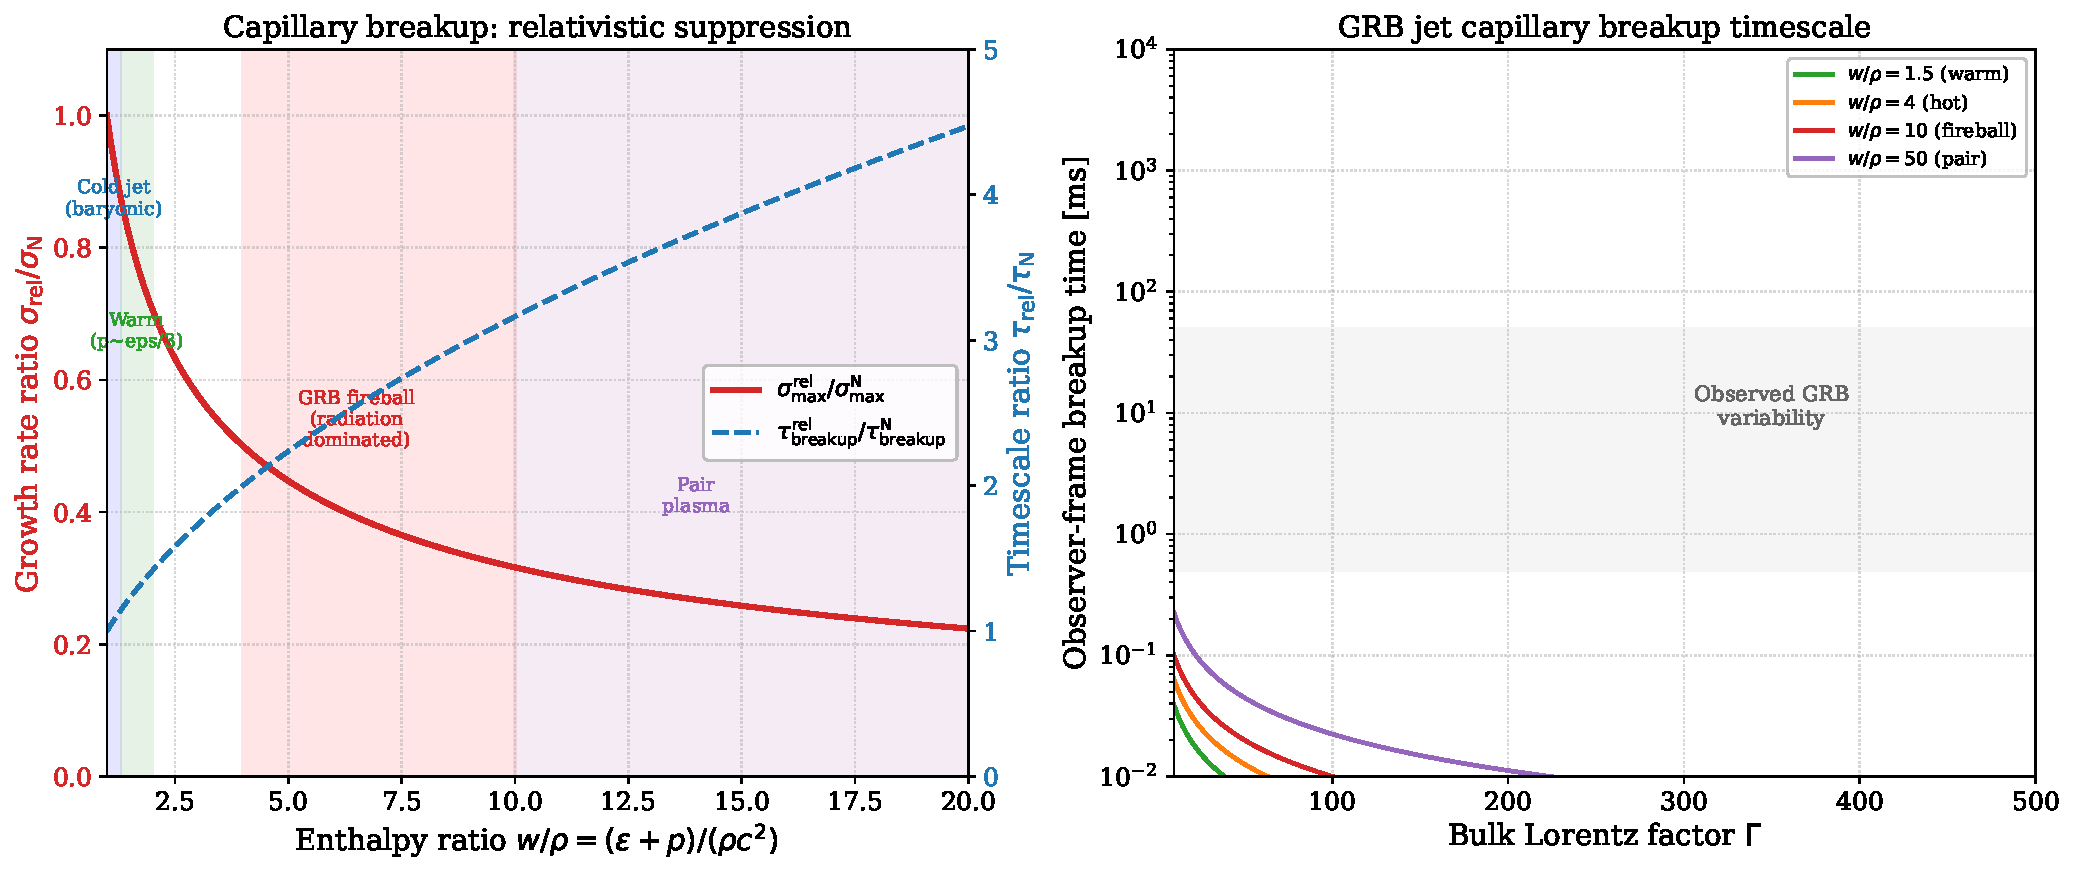
\includegraphics[width=0.95\textwidth]{plots/ch12/fig_jet_capillary_breakup.pdf}
\caption{%
\textbf{Left:} Relativistic suppression of the capillary growth rate
and enhancement of the breakup timescale as functions of the
enthalpy ratio $w/\rho = (\varepsilon+p)/(\rho c^{2})$, with
astrophysical regimes indicated.
\textbf{Right:} Observer-frame breakup timescale for a GRB jet
(cocoon-confined, $R=10^{7}\;\mathrm{cm}$) as a function of bulk
Lorentz factor $\Lf$, for several internal enthalpy ratios.  The
grey band marks the observed GRB variability range.}
\label{fig:jet-capillary-breakup}
\end{figure}

%% ===================================================================
\section*{BIBLIOGRAPHICAL NOTES (\S\S111--112)}
\label{sec:rel-12-111-112-bib}

The classical capillary instability was discovered by:
\begin{enumerate}
\item J.~\textsc{Plateau}, \emph{Statique exp\'erimentale et
  th\'eorique des liquides soumis aux seules forces
  mol\'eculaires}, Gauthier-Villars, Paris, 1873.

\item Lord~\textsc{Rayleigh}, `On the instability of jets',
  \emph{Proc.\ London Math.\ Soc.}\ \textbf{10}, 4--13 (1878).
\end{enumerate}

\noindent
Relativistic surface energy--momentum tensor and junction conditions:
\begin{enumerate}
\setcounter{enumi}{2}
\item W.~\textsc{Israel}, `Singular hypersurfaces and thin shells in
  general relativity', \emph{Nuovo Cimento B}, \textbf{44}, 1--14
  (1966).

\item E.~\textsc{Poisson}, \emph{A Relativist's Toolkit: The
  Mathematics of Black-Hole Mechanics}, Cambridge Univ.\ Press, 2004.
\end{enumerate}

\noindent
GRB jet structure and variability:
\begin{enumerate}
\setcounter{enumi}{4}
\item P.~\textsc{M\'esz\'aros}, `Gamma-ray bursts', \emph{Rep.\ Prog.\
  Phys.}\ \textbf{69}, 2259--321 (2006).

\item A.~\textsc{Bromberg} et al., `The propagation of relativistic
  jets in external media', \emph{Astrophys.\ J.}\ \textbf{740}, 100
  (2011).

\item O.~\textsc{Gottlieb} et al., `The structure of weakly
  magnetized gamma-ray burst jets', \emph{Astrophys.\ J.\ Lett.}\
  \textbf{933}, L9 (2022).
\end{enumerate}

\noindent
BDNK causal viscous theory:
\begin{enumerate}
\setcounter{enumi}{7}
\item F.~S.~\textsc{Bemfica}, M.~M.~\textsc{Disconzi}, and
  J.~\textsc{Noronha}, `Causality and existence of solutions of
  relativistic viscous fluid dynamics with gravity',
  \emph{Phys.\ Rev.\ D}, \textbf{98}, 104064 (2018).

\item P.~\textsc{Kovtun}, `First-order relativistic hydrodynamics is
  stable', \emph{J.\ High Energy Phys.}\ \textbf{2019}(10), 034 (2019).

\item R.~E.~\textsc{Hoult} and P.~\textsc{Kovtun}, `Stable and causal
  relativistic Navier--Stokes equations', \emph{J.\ High Energy Phys.}\
  \textbf{2020}(06), 067 (2020).
\end{enumerate}
